\documentclass{IEEEcsmag}

\usepackage{amsmath,amsfonts}
\usepackage{graphicx}
\usepackage{booktabs}
\usepackage[colorlinks,urlcolor=blue,linkcolor=blue,citecolor=blue]{hyperref}
\expandafter\def\expandafter\UrlBreaks\expandafter{\UrlBreaks\do\/\do\*\do\-\do\~\do\'\do\"\do\-}
\usepackage{upmath,color}

\jvol{XX}
\jnum{XX}
\paper{8}
\jmonth{Month}
\jname{IEEE MultiMedia}
\jtitle{IEEE MultiMedia}
\pubyear{2026}

\setcounter{secnumdepth}{0}

\begin{document}

\sptitle{Feature Article: Line-Art Gap Closing}

\title{InkCloser: Line-Art Completion for Paint-Bucket Colorization}

\author{Ruben Tous}
\affil{Universitat Polit\`ecnica de Catalunya, Barcelona, Spain}

\markboth{FEATURE}{FEATURE}

\begin{abstract}
Paint-bucket (flood-fill) coloring of line art requires closed regions, but drawings
often contain small gaps that let the fill leak into neighboring regions. We present
InkCloser, a deep network that finds and closes such gaps without being told where
they are, so that a standard bucket tool works without manual retouching. The
network combines gated convolutions with self-attention at two resolutions and is trained on 54,000 pairs of clean and synthetically broken coloring pages. Instead of pixel accuracy, we evaluate what matters
to an artist: whether gaps are closed and whether one click fills each region. On
1,000 test drawings, InkCloser closes 70.5\% of the gaps, raises the fraction of
correctly fillable regions from 64.1\% to 94.7\%, and makes 45.0\% of the drawings
leak-free, whereas morphological closing and a prior learned method do not improve on the input.
\end{abstract}

\maketitle

\chapteri{T}wo-dimensional cartoon and animation production relies heavily on line
art: dark strokes on a light background that delimit the regions of a drawing. These
regions are usually colored with a paint-bucket, or flood-fill, tool, which fills an
enclosed area in a single click. The tool has one strict requirement: the contours
must be closed. Wherever a stroke is interrupted, the fill escapes through the
opening and leaks into the neighboring region, often the background, so that a
single click colors half the drawing.

Gaps are common in practice. They appear when strokes are drawn quickly and stop
just short of the line they should touch, when drawings are scanned or compressed,
and when lines are thinned or extracted automatically from other images. Most
drawing applications offer a ``close gap'' option that treats openings below a
user-set size as closed. This helps with tiny gaps, but the threshold is a
trade-off: a low value lets wider gaps leak, and a high value also closes narrow
passages between nearby strokes that should stay open. As a result, artists still
spend time zooming in and repairing lines by hand before coloring.

In this article, we take a different route and repair the line art itself. Given a
drawing with interrupted strokes, our system, InkCloser, redraws the missing ink so
that every region is closed and can be filled with one click, without per-drawing
tuning (see Figure~\ref{fig:intro}). The repaired drawing is closed for any tool, so
the method complements, rather than replaces, the gap-closing options of existing
software.

\begin{figure*}
\centerline{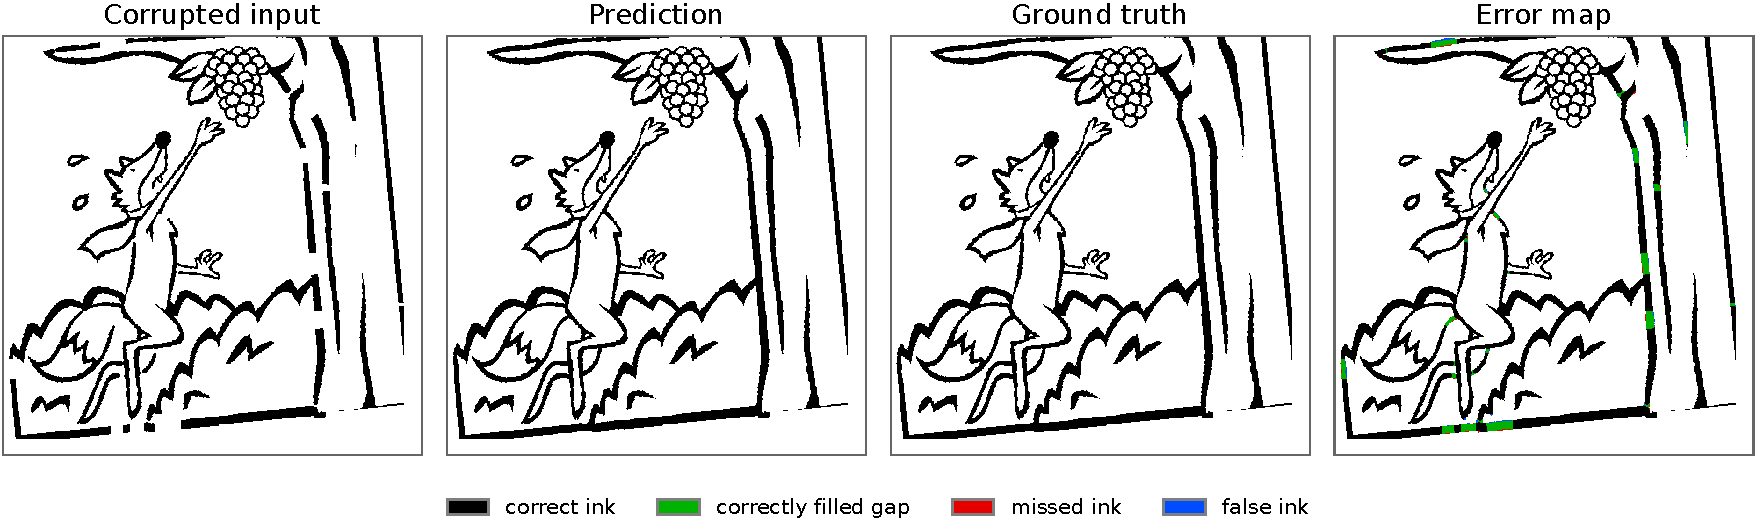
\includegraphics[width=\textwidth]{figures/pair_00000_intro.pdf}}
\caption{An example of line-art restoration. From left to right: the corrupted
input, with stroke segments missing; the output of InkCloser; the original drawing
(ground truth); and an error map comparing the two.}
\label{fig:intro}
\end{figure*}

The task resembles image inpainting, in which a network fills in a missing part of
an image, with one important difference: nobody tells the network where the gaps
are. It must find them and close them while leaving the rest of the drawing exactly
as it was. This is harder than it sounds, because not every open stroke end is a
defect. Line art is full of strokes that end on purpose, such as the folds of a
sleeve or the wrinkles around an eye. Whether an opening is a gap or an intentional
stroke ending cannot be decided from local geometry alone; it has to be learned from
many examples of complete, correctly closed drawings.

Our contributions are a network architecture that locates and bridges gaps without
a mask; a loss function that concentrates training on the missing strokes;
evaluation metrics that simulate the paint-bucket tool instead of counting correct
pixels; and a public dataset of 55,000 broken and clean line-art pairs~\cite{datasetInkCloser},
released together with the code and trained model~\cite{codeInkCloser}.

\section{HOW GAPS ARE HANDLED TODAY}

\textbf{Inpainting.} Learned image inpainting fills a masked region from its
surroundings. Modern networks handle irregular holes by tracking which input pixels
are valid~\cite{liu2018partialconv,yu2019gatedconv} and fill large holes using
image-wide context~\cite{suvorov2022lama}. All of these methods assume that the mask
of the missing region is given. Blind inpainting methods such as
VCNet~\cite{wang2020vcnet} first predict which pixels are corrupted, but they target
natural photographs, where damage looks like a foreign pattern. In line art, a gap is
simply missing ink, which looks exactly like background.

\textbf{Gap tolerance at coloring time.} The cartoon community has long dealt with
leaks without any learning. Morphological closing~\cite{serra1982morphology}, a
dilation of the ink followed by an erosion, bridges gaps up to the size of its
structuring element, but it also fills narrow background areas and sharp corners.
Trapped-ball segmentation~\cite{zhang2009vectorizing} floods the background with a
ball too large to pass through small gaps, LazyBrush~\cite{sykora2009lazybrush}
treats coloring from user scribbles as an optimization that tolerates small gaps,
and the method of Fourey et al.~\cite{fourey2018flat}, which underlies the line-art
mode of the bucket tool in GIMP, extends stroke endpoints with splines and segments.
Delaunay Painting~\cite{parakkat2022delaunay} propagates user color hints over a
triangulation of the contours and is robust to large gaps. These tools prevent leaks
at coloring time, but they either do not restore the missing strokes or close them
with hand-designed geometric rules and size thresholds. Recent work on the opposite
problem, small regions left unpainted after bucket filling~\cite{kono2026gapfill},
shows that the paint-bucket workflow is still an active research topic.

\textbf{Learned line-art restoration.} The closest work to ours is that of Sasaki et
al.~\cite{sasaki2017joint}, who train a fully convolutional network on synthetically
corrupted drawings to detect and fill gaps jointly, without a mask. Related cleanup
tasks, such as sketch simplification~\cite{simoserra2016simplify}, aim at visually
clean drawings. Our objective is different: we design and evaluate the system for
flood-fill coloring, that is, for whether regions end up correctly closed.

\textbf{Why closed regions matter downstream.} Recent learning-based tools for 2D
animation colorize a drawing region by region, for instance by matching the regions
of a frame to those of reference frames~\cite{casey2021animation,dai2024inclusion}.
For such tools, a single gap merges two regions and corrupts the color of both.
InkCloser can serve as a preprocessing step that supplies the closed contours these
tools assume.

\section{BUILDING A DATASET OF BROKEN DRAWINGS}

Training a network to close gaps requires pairs of broken and intact drawings. We
started from 10,000 clean, closed monochrome line-art images collected from
coloring-page collections, such as the Coloring Book Objects
dataset~\cite{chen2019human}. Coloring pages are ideal for this purpose, since they
are designed precisely to be filled region by region. Each image was resized to
$896\times 896$ pixels.

We then broke the drawings synthetically, working on the skeleton (the one-pixel-wide
centerline) of the strokes. A first step targets T-junctions, where one line meets
another: it erases the first few pixels of the arriving line, reproducing the common
hand-drawing defect of a stroke that stops just short of its target. A second step
cuts gaps in the middle of strokes. To keep the drawings recognizable, no more than
35\% of a stroke and 25\% of a connected shape is removed, and small shapes such as
eyes or highlights are never touched.

The images were split into 9,000 for training and 1,000 for testing. Each training
image has six differently broken versions, one of which is picked at random every
time the image is used, so the network sees varied gap patterns for the same drawing.
Each test image has a single fixed broken version, so every method we compare is
evaluated on exactly the same gaps. In total, the InkCloser dataset contains 55,000
pairs. During training, both images of a pair also undergo the same random flips,
small rotations, translations, and scalings.

\section{THE INKCLOSER NETWORK}

Figure~\ref{fig:overview} shows the architecture. Its backbone is a U-Net~\cite{ronneberger2015unet}:
an encoder progressively reduces the image from $896\times 896$ to $28\times 28$
pixels while increasing the number of feature channels from 16 to 512, and a decoder
brings it back to full resolution. Skip connections pass the encoder features at each
resolution directly to the decoder, which makes it easy for the network to copy
intact strokes to the output unchanged. This matters, because any stroke the network
weakens becomes a new gap.

\begin{figure*}
\centerline{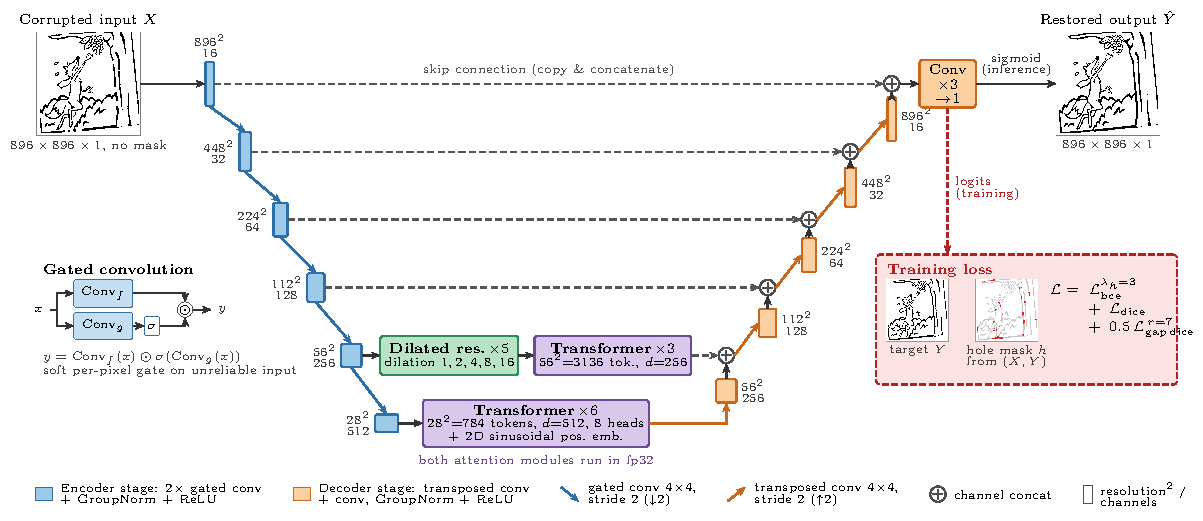
\includegraphics[width=\textwidth]{figures/fig_diagram.pdf}}
\caption{Architecture of InkCloser. The corrupted image is processed without a hole
mask by a U-Net whose encoder uses gated convolutions. Global context is added by six
transformer blocks at the $28\times 28$ bottleneck and by a dilated residual stack
followed by three transformer blocks on the $56\times 56$ skip connection. The
training loss (dashed) uses the target and the hole mask derived from the
input-target pair. Numbers next to each block give resolution$^2$ and channels.}
\label{fig:overview}
\end{figure*}

\textbf{Gated convolutions.} Every convolution in the encoder is a gated
convolution~\cite{yu2019gatedconv}. Besides its usual output, each such layer
computes a ``gate'' between 0 and 1 for every position and multiplies the two. In
effect, the network learns at every layer and location how much to trust each part
of its input, which suits a task in which some parts of the input, the gaps, are
unreliable by construction.

\textbf{Seeing the whole drawing.} A stack of small convolutions sees only a limited
neighborhood of each pixel, but gaps can be long. To decide how a stroke should
continue, the network needs to see both of its ends and the shape around them. We
therefore add two modules that provide image-wide context. At the bottleneck, the
$28\times 28$ grid of features is treated as a sequence of 784 tokens and processed
by six transformer blocks~\cite{vaswani2017attention}, whose self-attention lets every
position exchange information with every other position, however far apart. At the
$56\times 56$ level, the features passed through the skip connection first go through
five residual blocks with increasingly spaced (dilated) convolutions, which widen the
receptive field cheaply, and then through three more transformer blocks. This gives
the decoder global context at a finer resolution than the bottleneck.

The network outputs, for each pixel, the probability that it is background; the
restored drawing is obtained by thresholding this map at 0.5. The model has 43.4
million parameters.

\section{TEACHING THE NETWORK TO FOCUS ON GAPS}

A naive training loss would teach the network very little about gaps. Ink covers only
a small fraction of a drawing, and the missing ink an even smaller one, so a network
that simply copies its input already looks nearly perfect pixel by pixel. We
therefore combine three terms. Because the training pairs tell us exactly which
pixels were erased, we can use this ``hole mask'' during training, even though it is
not available at inference time.

The first term is a standard pixel-wise cross-entropy against the clean drawing, in
which erased pixels count three times as much as the others. The second is a Dice
loss~\cite{milletari2016vnet}, which measures the overlap between predicted and true
ink over the whole image and is insensitive to how much background there is. The
third applies the same Dice loss only to a 15-pixel-wide neighborhood around the
erased segments, so that the network is rewarded specifically for completing the
strokes, regardless of how well it reproduces the rest of the image. In early
experiments, weighting erased pixels much more heavily made the network add spurious
ink around the gaps; the combination above balances closing gaps against preserving
the drawing.

The network was trained for five epochs with the AdamW optimizer, mixed-precision
arithmetic, and a batch size of four.

\section{MEASURING WHAT ARTISTS CARE ABOUT}

Pixel accuracy is a poor measure of success here. A method that adds no ink at all
already scores 98.4\% pixel F1 on our test set, because the gaps are a tiny part of
the image, and pixel overlap says nothing about whether regions are closed. We
therefore measure quality at three levels.

\textbf{Added ink.} \emph{Fill F1} considers only the pixels that a method adds: it
combines the fraction of added ink that lies on the true strokes (precision) with the
fraction of erased ink that was redrawn (recall). The \emph{ink ratio}, the total
output ink divided by the true ink, reveals whether strokes are systematically too
thick (above 1) or too thin (below 1).

\textbf{Gaps.} Each connected piece of erased ink is one gap; there are 26,141 in the
test set. A gap counts as closed if at least 80\% of its pixels are ink in the
output. \emph{Gap closure} is the fraction of closed gaps.

\textbf{Paint-bucket behavior.} These metrics simulate the coloring tool directly.
Each region of the original drawing is matched to the output region that overlaps it
best, and is counted as correctly fillable if their overlap (intersection over
union) is at least 0.9. \emph{Bucket accuracy} is the fraction of correctly fillable
regions, roughly the fraction of regions a user could color with one click. A
\emph{leak} occurs when one output region swallows most of two original regions, so
that a single click would spill across them. We report the average number of leaks
per image and the fraction of \emph{leak-free} drawings, which are ready to color
without any manual correction.

We compare InkCloser with three baselines, all of which, like our method, receive
only the broken image. The unrestored input shows how much damage the gaps cause.
Morphological closing with a 5- or 9-pixel structuring element is the classical
training-free remedy and essentially what the ``close gap'' option of drawing software
does. Finally, the joint gap detection and inpainting network of Sasaki et
al.~\cite{sasaki2017joint} is evaluated in two ways: with its publicly released
weights, which we converted to PyTorch, and retrained from scratch on our training
data with the same augmentation as our model, following the original training
recipe. All methods are evaluated on the same 1,000 test drawings with the same code.
To check that differences are not due to chance, we use a paired bootstrap over the
test images.

\section{RESULTS}

Table~\ref{tab:results} summarizes the results. The metrics that capture the actual
goal of the task show the largest effect. On the unrestored input, only 64.1\% of the
regions can be filled correctly with one click, each drawing has 15.5 leaks on
average, and only one of the 1,000 drawings is leak-free. After restoration with
InkCloser, bucket accuracy rises to 94.7\%, leaks drop by 90.5\% to 1.5 per image, and
45.0\% of the drawings are entirely leak-free. Two-thirds of the restored drawings
have at most one leak, compared with a median of 13 before restoration. InkCloser is
the only method that improves the bucket accuracy of the input; every other method
lowers it. All of its improvements over each baseline in fill F1, gap closure, bucket
accuracy, and leak-free drawings are statistically significant (paired bootstrap,
$p\le 0.001$).

\begin{table*}
\caption{Results on the 1,000 test drawings (percentages, except the ink ratio and
the leaks per image). Fill F1: accuracy of the added ink. Ink ratio: output ink
divided by true ink (ideal: 1). Bucket acc.: regions fillable correctly with one
click. Best values in bold.}
\label{tab:results}
\tablefont
\begin{tabular*}{\textwidth}{@{\extracolsep{\fill}}lcccccc@{}}
\toprule
Method & Fill F1 & Ink ratio & Gap closure & Bucket acc. & Leaks/image & Leak-free \\
\midrule
Input (no restoration)      & --            & 0.968          & 0.0           & 64.1          & 15.46         & 0.1 \\
Closing (5 pixels)          & 1.4           & 1.021          & 1.4           & 37.6          & 13.08         & 0.2 \\
Closing (9 pixels)          & 2.1           & 1.129          & 6.3           & 22.8          & 9.45          & 0.3 \\
Sasaki et al. (pretrained)  & 17.8          & 1.081          & 26.6          & 26.2          & 13.77         & 4.2 \\
Sasaki et al. (retrained)   & 37.6          & 0.974          & 20.8          & 36.4          & 19.36         & 8.5 \\
InkCloser                   & \textbf{78.5} & \textbf{1.004} & \textbf{70.5} & \textbf{94.7} & \textbf{1.47} & \textbf{45.0} \\
\bottomrule
\end{tabular*}
\end{table*}

\textbf{Closing the gaps without damaging the drawing.} InkCloser redraws 84.0\% of
the erased ink exactly, and 73.6\% of the ink it adds lies exactly on the true
strokes. Allowing a tolerance of two pixels raises both figures above 91\%, so most of
the remaining error is a matter of stroke thickness or position rather than missing
or invented structure. Just as important, the model leaves the rest of the drawing
alone: it keeps 99.9998\% of the ink already present in the input, and its ink ratio
of 1.004 shows that restored lines are neither too thick nor too thin.

\textbf{Why morphological closing fails.} With a 9-pixel element, closing bridges
only 6.3\% of the gaps. It does reduce the number of leaks, but mostly by filling
narrow background areas and thickening junctions, which destroys small regions
instead of separating merged ones. Its bucket accuracy drops to 22.8\%, well below
that of the unrestored input. The 5-pixel element damages the drawing less, but
closes almost no gaps. Both effects are visible in Figure~\ref{fig:qualitative},
where closing merges nearby strokes into ink blobs while leaving most gaps open.

\textbf{Why redrawing everything is not enough.} The network of Sasaki et al.\
performs much better than closing at the ink level, but it does not make the drawings
paintable. With its released weights, it closes 26.6\% of the gaps, the most among the
baselines, but it redraws the whole drawing in the style of its own training data,
with thicker strokes and small spurious marks. Retrained on our data, it adopts the
right line style, yet its gap closure falls to 20.8\% and the number of leaks rises
to 19.4 per image, more than in the unrestored input. The reason is that this network
regenerates every stroke instead of copying the input where it is intact: it keeps
only 94.1\% of the input ink, thin strokes are partly lost, and every weakened stroke
opens a new gap. Since this variant uses the same data and augmentation as ours, the
difference, 49.7 percentage points in gap closure and 58.4 in bucket accuracy,
reflects the architecture and training objective. We attribute it to the skip
connections and gated convolutions, which let intact strokes pass through unchanged,
and to the attention modules and gap-focused loss, which focus the network's capacity
on the gaps.

\begin{figure*}
\centerline{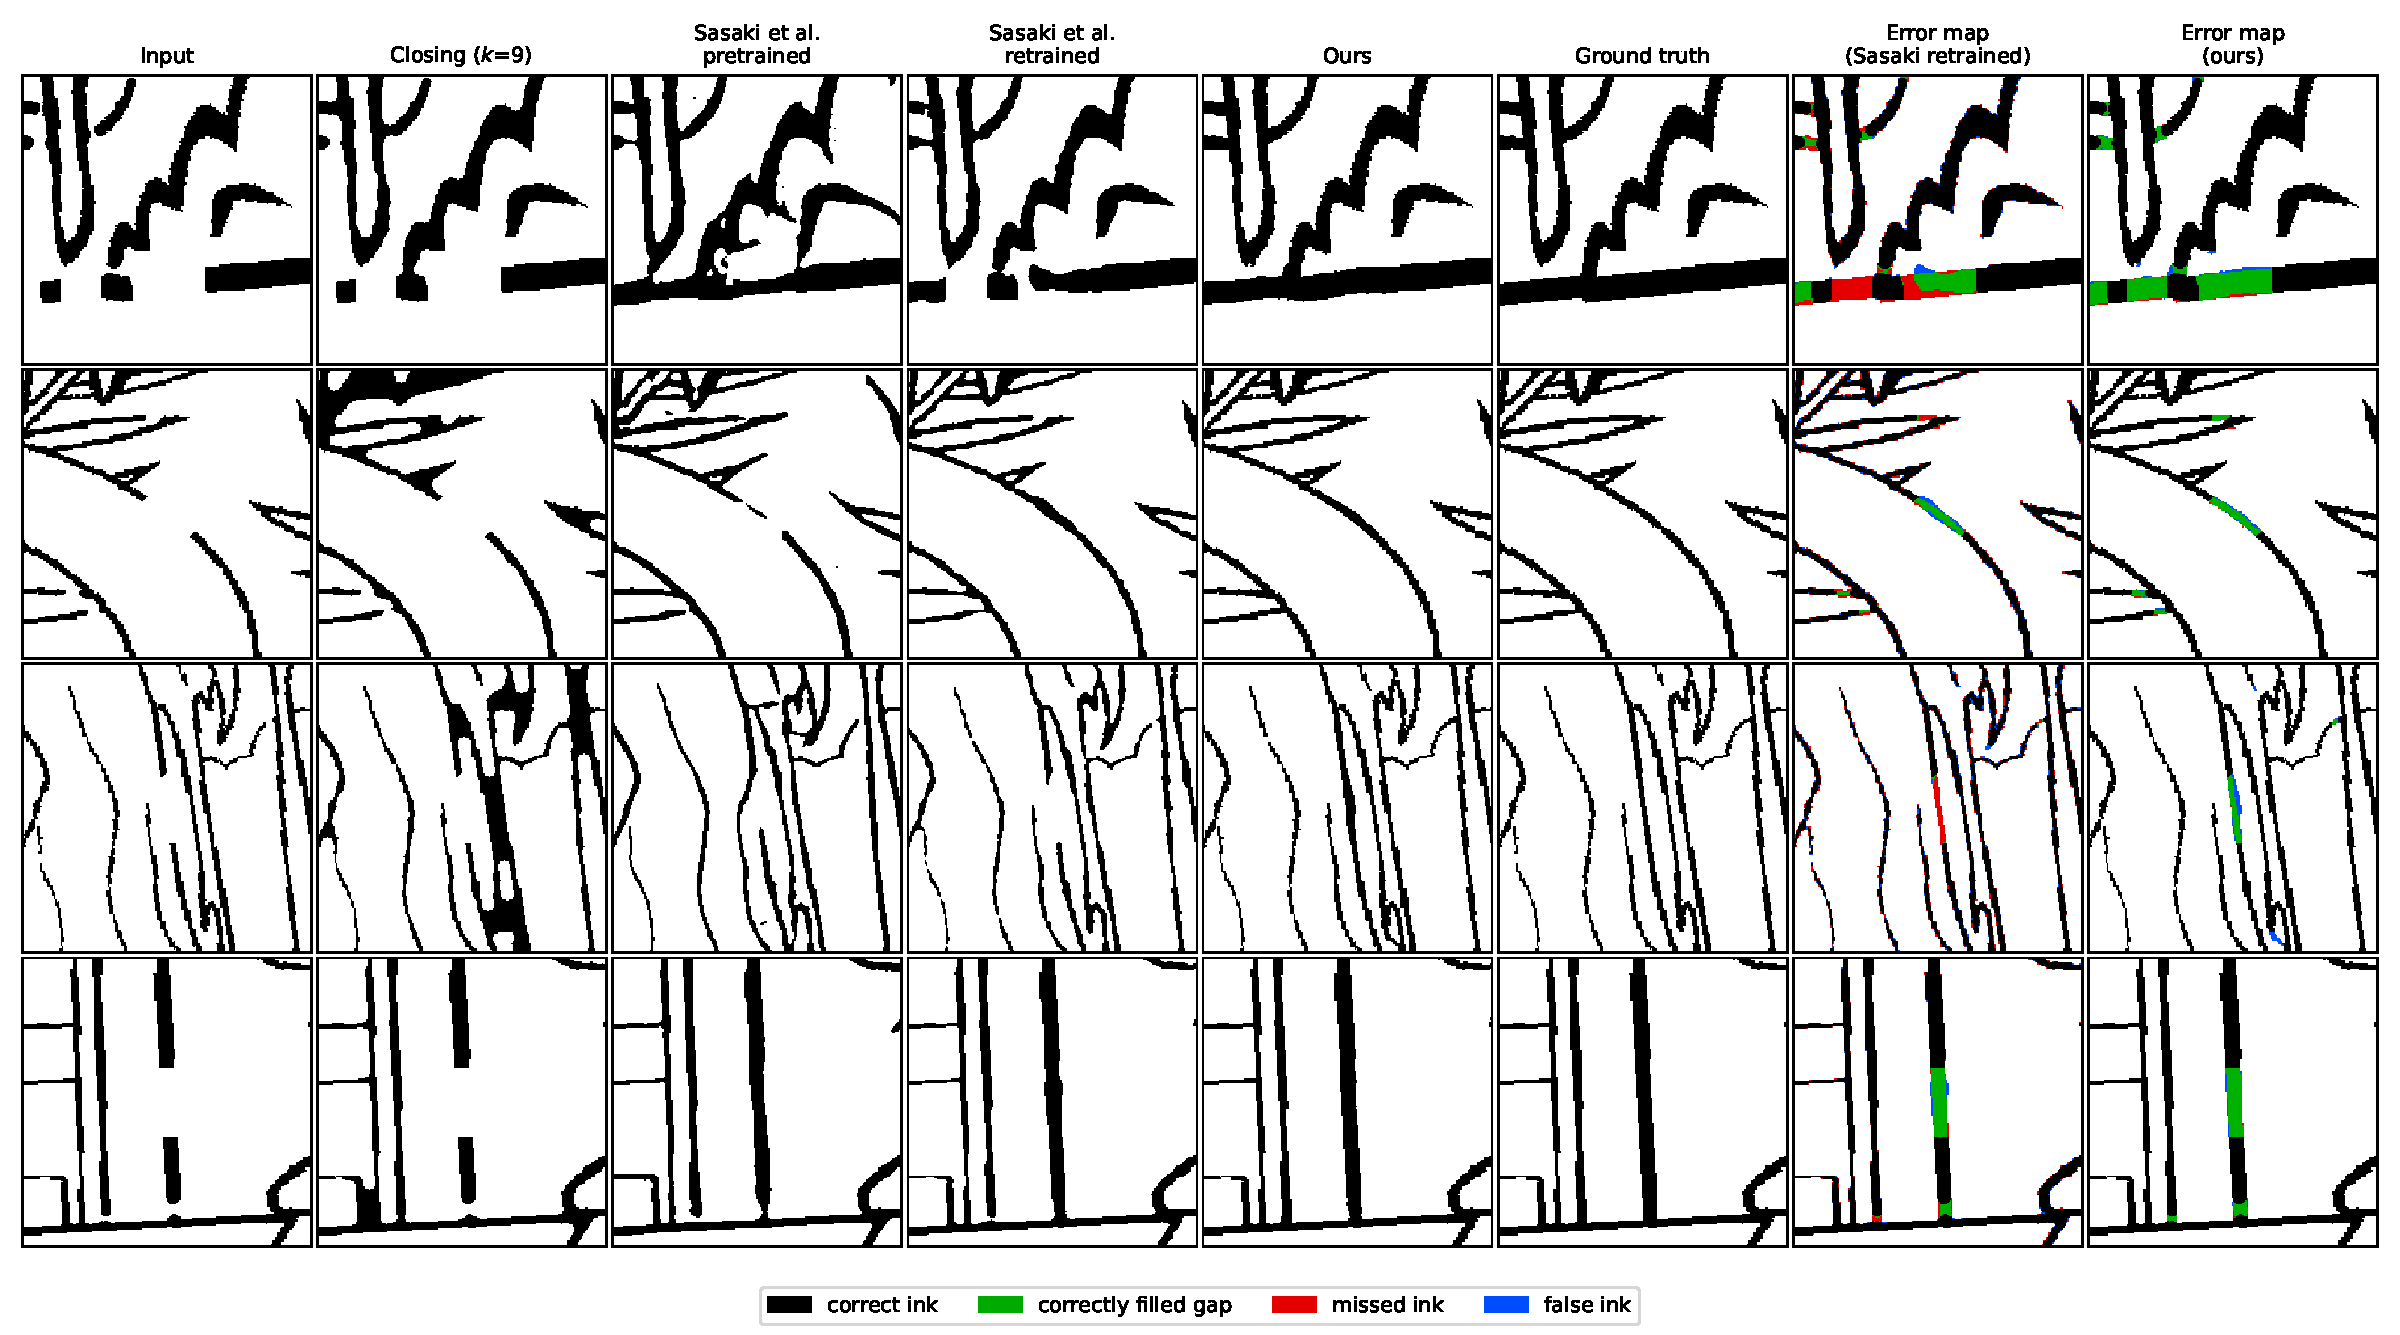
\includegraphics[width=\textwidth]{figures/fig_qualitative_zoom_all.pdf}}
\caption{Close-ups of four test drawings, centered on their largest gap. Columns:
broken input, morphological closing (9 pixels), the pretrained and retrained network
of Sasaki et al., InkCloser, the original drawing, and the error maps of the retrained
Sasaki et al.\ network and of InkCloser (black: correct ink; green: erased ink
correctly redrawn; red: missed ink; blue: false ink).}
\label{fig:qualitative}
\end{figure*}

\textbf{Long gaps.} Figure~\ref{fig:gaplength} breaks down gap closure by gap length.
Morphological closing only handles gaps shorter than its structuring element, and
practically none above 16 pixels. The Sasaki et al.\ network closes at most 43\% of
the gaps in any length range. InkCloser closes between 76.6\% and 80.0\% of the gaps
in every range from 8 pixels upwards, including 12 of the 15 gaps longer than 64
pixels, which is consistent with the image-wide context provided by its attention
modules. Its closure rate is lowest, 44.5\%, for gaps under 8 pixels, although it is
still the best of all methods there. We believe this is largely an effect of the
closure criterion: for a gap of a few pixels, a completion that is one pixel thinner
or offset fails to cover 80\% of it, whereas the same error is negligible for a long
gap.

\begin{figure}
\centerline{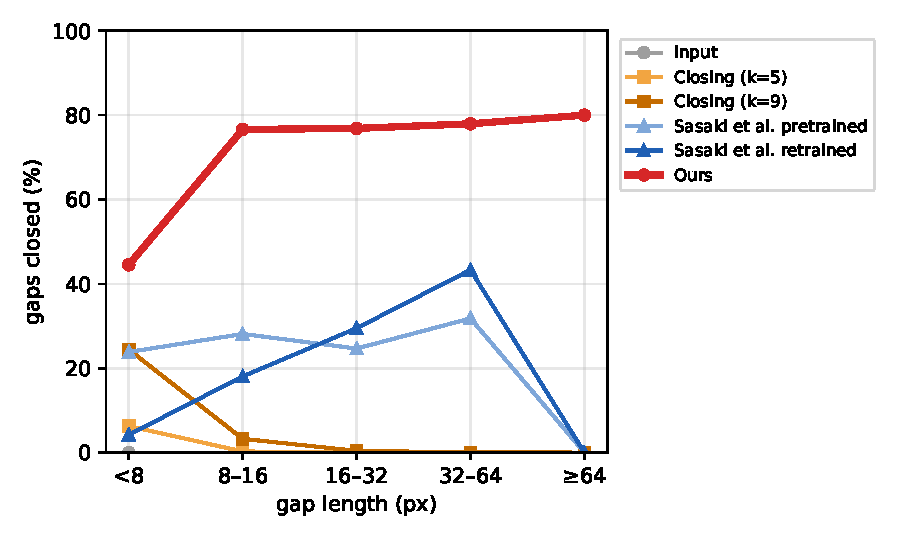
\includegraphics[width=\columnwidth]{figures/fig_gap_closure_by_length_all.pdf}}
\caption{Fraction of gaps closed by each method as a function of gap length (longer
side of the gap's bounding box). The last bin contains only 15 gaps.}
\label{fig:gaplength}
\end{figure}

\textbf{Visual quality and failures.} In Figure~\ref{fig:qualitative}, InkCloser
reconstructs long stretches of straight and curved strokes with the correct
thickness and continues strokes through junctions; its few errors are mostly
one-pixel deviations along the completed strokes. Its main failure mode is a long
missing stretch of a curved contour whose shape cannot be inferred from its ends,
such as the lobe of a leaf. In those cases, the model leaves the gap open rather
than guessing, and so does the retrained Sasaki et al.\ network. Areas with many
close, nearly parallel strokes or fine hatching are also harder: some strokes are
completed only partially. Even then, InkCloser does not produce the ink blobs that
closing creates.

\textbf{Speed.} Restoring one $896\times 896$ drawing takes 92 ms in half precision
on an NVIDIA T4 GPU, with 1.24 GB of peak GPU memory. This is roughly an order of
magnitude more than the much smaller Sasaki et al.\ network, but fast enough for an
interactive preprocessing step before coloring, and small compared with the cost of
repairing gaps by hand.

\section{LESSONS AND LIMITATIONS}

The main lesson of this work is that closing gaps visually is not enough for
coloring. A method that regenerates the whole drawing can recover much of the
missing ink and still produce more leaks than it started with, because every stroke
it weakens elsewhere becomes a new gap. For a paint-bucket workflow, preserving the
input exactly outside the gaps is as important as filling them, and evaluation should
count leaks and fillable regions rather than pixels.

Several limitations remain. Although InkCloser separates 94.0\% of the regions merged
by gaps, a single remaining gap is enough to spoil a fill, and 55\% of the restored
drawings still contain at least one leak. From an artist's point of view, however,
the remaining work drops from about 15 corrections per drawing to one or two in most
cases. Weighting the loss towards gaps that actually merge regions, and improving the
closure of very short gaps, are direct ways to raise the fraction of leak-free
drawings. All our results were obtained with synthetic gaps in coloring pages at a
single resolution. Real gaps caused by scanning, compression, or line thinning may
differ in shape and size, and the modest zero-shot results of the pretrained Sasaki
et al.\ network on our data show how strongly such models can depend on their
training data. Validating the approach on naturally occurring gaps and on other line
styles, resolutions, and stroke widths is the next step of this work.

\section{CONCLUSION}

InkCloser restores broken lines in line art so that a standard paint-bucket tool can
color the result with single clicks. It finds and closes gaps without being told
where they are, and it leaves the rest of the drawing untouched. On 1,000 test
drawings, it closes 70.5\% of the gaps, makes 94.7\% of the regions fillable with one
click, and turns 45\% of the drawings into leak-free line art, while neither
morphological closing nor a prior learned approach improves on the unrestored input.
The code, trained model, and dataset are publicly
available~\cite{codeInkCloser,datasetInkCloser}, and we hope they will help make gap
repair an automatic step in digital coloring pipelines.

\section{ACKNOWLEDGMENTS}

This work has been financed by Project PID2024-160996OB-I00, under grant agreement
MICIU/AEI/10.13039/501100011033 and FEDER, UE, and by Generalitat de Catalunya
(AGAUR) under grant agreement 2021-SGR-00478.

\def\refname{REFERENCES}
\bibliographystyle{IEEEtran}
\bibliography{references}

% Biography with photo. The class's optional photo argument of IEEEbiography does not
% work, so the photo and the text are set side by side in the class's biography font.
\vspace{2\baselineskip}
\noindent
\begin{minipage}[t]{1in}\vspace{0pt}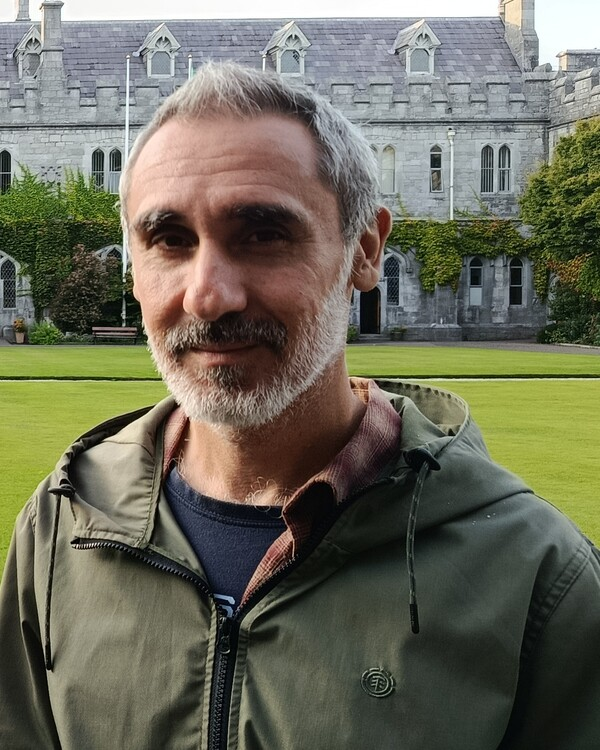
\includegraphics[width=1in,height=1.25in,keepaspectratio]{figures/rtous.jpg}\end{minipage}\hfill
\begin{minipage}[t]{\dimexpr\columnwidth-1.14in\relax}\vspace{0pt}\sffamily\fontsize{9}{12}\selectfont
\textbf{Ruben Tous} is an associate professor with the Department of Computer
Architecture, Universitat Polit\`ecnica de Catalunya, Barcelona, Spain. His research
interests include computer vision, image and video synthesis, and artificial
intelligence for animation. He received the Ph.D. degree in computer science and
digital communication from Pompeu Fabra University. Contact him at
ruben.tous@upc.edu.
\end{minipage}

\end{document}
